\normalfalse \difficilefalse \tdifficiletrue
\correctionfalse

%\UPSTIidClasse{11} % 11 sup, 12 spé
%\newcommand{\UPSTIidClasse}{12}

\exer{Maxpid $\star\star\star$ \label{C2:09:18}}
\setcounter{question}{0}\UPSTIcompetence[2]{C2-09}
\index{Compétence C2-09}
\index{TEC}
\index{Théorème de l'énergie cinétique}
\index{Maxpid}
\ifcorrection
\else
\marginnote{\textbf{Pas de corrigé pour cet exercice.}}
\fi

\ifprof
\else

Soit le schéma suivant. 
\begin{center}
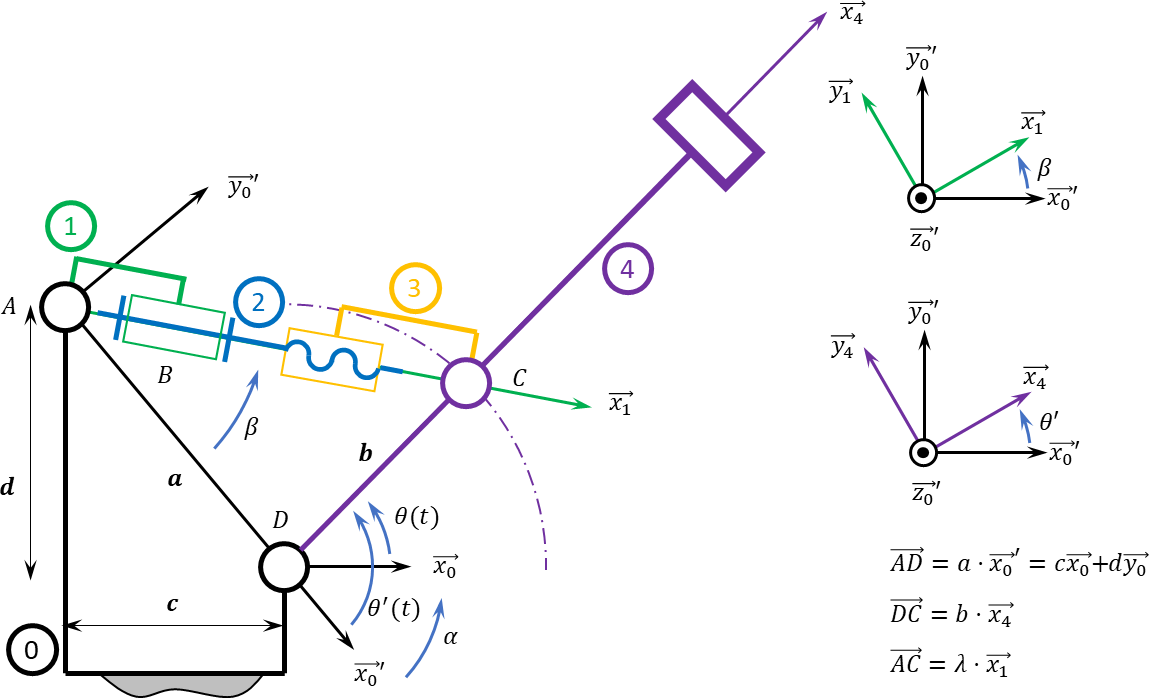
\includegraphics[width=\linewidth]{18_01}
\end{center}


Par ailleurs $a=\SI{107,1}{mm}$, $b=\SI{80}{mm}$, $c=\SI{70}{mm}$, $d=\SI{80}{mm}$. Le pas de la vis est de $\SI{4}{mm}$. De plus, on note :
\begin{itemize}
\item $G_1=B$ le centre d'inertie du solide \textbf{1}, $m_1$ sa masse et $\inertie{G_1}{1}=\matinertie{A_1}{B_1}{C_1}{0}{0}{0}{\rep{1}}$ sa matrice d'inertie;
\item $G_2$ le centre d'inertie du solide \textbf{2} tel que $\vect{BG_2}=L\vx{1}$, $m_2$ sa masse et $\inertie{G_2}{2}=\matinertie{A_2}{B_2}{C_2}{0}{0}{0}{\rep{2}}$ sa matrice d'inertie;
\item $G_3=C$ le centre d'inertie du solide \textbf{3}, $m_3$ sa masse et $\inertie{G_3}{3}=\matinertie{A_3}{B_3}{C_3}{0}{0}{0}{\rep{3}}$ sa matrice d'inertie;
\item $G_4$ le centre d'inertie du solide \textbf{4} tel que $\vect{DG_4}=L_4\vx{4}$, $m_4$ sa masse et $\inertie{G_4}{4}=\matinertie{A_4}{B_4}{C_4}{0}{0}{0}{\rep{4}}$ sa matrice d'inertie;.
\end{itemize}
On note $C_m\vk{0}$ le couple moteur agissant sur le solide \textbf{1}. L'accélération de la pesanteur est donnée par $\vect{g}=-g\vy{0}$.
On rappelle que la loi entrée sortie est donnée par la relation *** établie à l'exercice \ref{C2:06:17}.

\fi

\question{Tracer le graphe d'analyse en indiquant l'ensemble des actions mécaniques agissant sur les différents solides.}
\ifprof
\else
\fi

\question{Déterminer l'ensemble des puissances intérieures à l'ensemble \textbf{1+2+3+4}.}
\ifprof
\else
\fi

\question{Déterminer l'ensemble des puissances extérieures à l'ensemble \textbf{1+2+3+4}.}
\ifprof
\else
\fi

\question{Déterminer $\ec{1+2+3+4}{0}$.}
\ifprof
\else
\fi

\question{Déterminer la loi de mouvement en appliquant le théorème de l'énergie cinétique.}
\ifprof
\else
\fi

\ifprof
\else
\begin{flushright}
\footnotesize{Corrigé  voir \ref{C2:09:18}.}
\end{flushright}%
\fi